\section{Update Governance}

%\paragraph{What is update governance. Why we should care?}
With the term \emph{update governance} we mean the processes used to control the software updates mechanism. %As we have seen, in the centralized setting, update governance is quite straightforward.
In the centralized setting, the mere existence of a central authority (owner of the code) simplifies decision making significantly. On the other side, in the decentralized approach, we have seen that all decision-making procedures have been replaced by a voting process, where a decision is taken collectively by the whole stake. Thus, we are dealing with a \emph{decentralized governance model}. Therefore voting and delegation are key components of a decentralized approach to software updates.
%\paragraph{What is the scope of the sections that follow?}
%It is true that in the decentralized setting the tools that one has at one's
% disposal for controlling the software updates process, but more importantly,
% for leading the participating stakeholders towards an \emph{update consensus},
% i.e., to reach at an agreement regarding the acceptance, or not, of the
% updates and the order (i.e., priorities), by which these will be applied, are
% the voting and delegation mechanisms.
In this section, we describe both of these mechanisms.
% and end with a description of the software updates protocol that encompasses them.


\subsection{Voting for Software Updates} \label{appxvoting}

\subsubsection{Voting for SIPs and UPs}
%Voting is the main vehicle for driving democracy and in our case is indeed the main mechanism for decision making in a decentralized setting for software updates. During the lifecycle of a software update, we have identified two phases, where a voting process is required. The first appears in the ideation phase and has to do with the approval of SIPs, while the second lies in the approval phase and deals with the approval of submitted source code and metadata (optionally binaries also), namely the UP bundle. Apart from the fact that the object of the voting process differs in these two phases, everything else is the same, so in the text that follows, whatever we describe, pertains to both of the voting phases, unless explicitly specified.

Voting is the main vehicle for driving democracy and in our case is indeed the main mechanism for decision making in a decentralized setting for software updates
%\paragraph{What is a vote}
\emph{A vote} is a fee-based transaction that is valid for a specific period of time called the \emph{voting period}. In particular, after the object of voting (a SIP or a UP) has been submitted to the blockchain (initially encrypted and then at a second step revealed - based on a commit-reveal scheme),% it has been buried under a sufficient number of blocks, in order to be confirmed and finally it has been revealed,
then the voting period for this software update begins.

We acknowledge the fact that not all software updates are equal and therefore, we cannot have a fixed voting period. %Moreover, software updates (especially UPs, which are essentially source code) are complex technical objects, where sufficient time must be provided for their evaluation.
Therefore, the voting period must be adaptive to the complexity of the specific software update. We propose to have a \emph{metadata-driven} voting period duration, based on the size, or complexity, of the software update.%, expressed as required man-effort in the accompanying metadata of the software update. %So the voting period duration $v_{duration}(su_{size})$ , which can be expressed as a number of blocks (or slots), is a function of the software update size (e.g., expressed in man-days).

We introduce a \emph{vote} as a new transaction type, the \emph{Software Update Vote Transaction (SUVT)} that can only be included in a block during the voting period (see Appendix~\ref{se:bcabstraction} for a formal definition of a transaction). The core information conveyed by the vote transaction (i.e., included into the transaction Payload field) is summarized in the following tuple:
$$( H(<SIP/UP>),SU_{Flag},<confidence>,vks_{source},\sigma_{sks_{source}}(m))$$
%\begin{align*}
%$( H(<SIP/UP>), \\
%  SU_{Flag}, \\
%  <confidence>, \\
%  vks_{source}, \\
% \sigma_{sks_{source}}(m))$
%\end{align*}
$H(<SIP/UP>$ is the hash of the content of the SIP/UP and plays the role of the unique id of a software update. $SU_{Flag}$ is a boolean flag (SIP/UP), which discriminates an SIP vote from an UP vote. $<confidence>$ is the vote per se, expressed as a three-valued flag (for/against/abstain). $vks_{source}$ is the public key of the party casting the vote. Finally, $\sigma_{sks_{source}}(m)$ is the cryptographic signature, signed with the private key corresponding to $vks_{source}$, on the transaction text $m$ (see Appendix~\ref{se:bcabstraction} for a formal definition of a signature scheme).

Anyone who owns stake has a legitimate right to vote and this vote will count proportionally to the owned stake. Furthermore, as we will describe in detail in the next section, the right to vote can also be delegated to another party. However, we want to give the power to a stakeholder to override the vote of his/her delegate. Therefore, if within the same voting period appear both a private vote and a delegate's vote, for the same software update, then the private vote will prevail.

%Moreover, as we have stated above, we acknowledge the fact that software updates are complex entities and their evaluation is a challenging task. This is true especially, when someone has to evaluate source code. Therefore,
Moreover,we cannot exclude the possibility that a voter/evaluator changes his/her mind after voting for a specific SU (for example, the evaluator identifies a software bug after voting positively for a software update). We want to provide the flexibility to the evaluators to change their minds. Therefore, we allow for a voter to vote multiple times, within a voting period for a specific software update. At the end, we count only the last vote of a specific public key in the voting period for a specific software update.

\subsubsection{Voting Results}
After the end of the voting period for a specific software update and after we allow some stabilization period (in order to ensure that all votes have been committed into the blockchain), the votes are tallied and an outcome is decided. First, the non-delegated votes are counted. The tallying is performed as follows: For each slot within the voting period, if a block was issued pertaining to that slot, each SUVT in that block is examined. If the staking key for that transaction has been tallied on a non-delegated vote previously, the previous vote is discarded and the new vote is counted. This allows voters to modify their votes until the end of the voting period. For every SUVT which has been counted, the stake that votes for it is summed and this constitutes the \emph{non-delegated stake in favour}, the \emph{non-delegated stake against} and the \emph{non-delegated abstaining stake}.

Subsequently, the delegated votes are counted. %For each slot within the voting period, if a block was issued pertaining to that slot, each SUVT in that block is examined.
If the delegatee staking key for that transaction has been tallied on a delegatable vote previously, the previous vote is discarded and the new vote is counted. For each of the delegatable votes, the keys delegating to it are found. Each of the keys delegating is checked to ensure that the delegating key has not cast a non-delegated vote; if the delegating key has also cast a non-delegated vote, then the non-delegated vote is counted instead of the delegated vote. For each delegatable SUVT which has been counted, the stake delegating to it which hasn't issued a non-delegated vote is summed and this constitutes the \emph{delegated stake in favour}, the \emph{delegated stake against}, and the \emph{delegated abstaining stake}.

The sum of the non-delegated stake in favour and delegated stake in favour forms the \emph{stake in favour}; similarly, we obtain the \emph{stake against} as well as the \emph{abstaining stake}.

%Suppose that the \emph{honest stake threshold assumption} of our software updates protocol is $h$
Suppose that we define a voting threshold $\tau_V$, then at the end of the tallying, a software update (i.e., a SIP or an UP) is marked one of the following:
\begin{itemize}

\item \emph{Approved}. When the $stake\ in\ favour > \tau_V$

\item \emph{Rejected}. When the $stake\ against > \tau_V$

\item \emph{No-Quorum}. When the $abstaining\ stake > \tau_V$. In this case, we revote (i.e., enter one more voting period) for the specific software update. This revoting can take place up to $rv_{no-quorum}$ times, which is a protocol parameter. After that, the software update becomes \emph{expired}.

\item \emph{No-Majority}. In this case none of the previous cases has appeared. Essentially, there is no majority result. Similarly, we revote (i.e., enter one more voting period) for the specific software update. This revoting can take place up to $rv_{no-majority}$ times, which is a protocol parameter. After that, the software update becomes expired.

\item \emph{Expired}. This is the state of a software update that has gone through $rv_{no-quorum}$ (or $rv_{no-majority}$) consecutive voting periods, but still it has failed to get approved or rejected.
\end{itemize}

In our proposal, we have chosen a three-value logic for our vote (for/against/abstain). In this way, apart from the actual result, we can extract the real sentiment (positive, negative, neutral) of the community for a specific software update. This is very important in a decentralized governance model, because it clearly shows the appeal of a software update proposal to the stakeholders. If we did not allow negative votes, then the negative feeling would be hidden under the abstaining stake.
%Moreover, the \say{abstain} vote is a sign that the stakeholder has not formed an opinion for, or against, a specific software update. However, it might also denote that the evaluator has not made yet a decision and maybe he/she needs more time. Therefore,
Moreover, the abstain vote can be also used as a way for the evaluator to say that the evaluation of the SU has not finished, a conclusion can not be drawn yet and indirectly submit a request for a time extension (i.e., a new voting period).

\begin{comment}
\subsection{Voting Threshold Analysis}
Lets assume that $H$ is the percent of honest stake and $T$ is the percent of 
adversarial stake that actively participate in the voting process. We assume 
also that
\begin{equation}\label{eq:H_plus_T}
	H+T=100    
\end{equation}
Moreover, the stake considered during the tally is the stake that the voters 
have at that moment. That is, we only consider the stake of the voters at the 
moment of the tally, without taking into account the stake that the voters had 
in the moment that the votes were casted. In other words, the calculation of 
the 
voting result corresponds to the stake distribution at the same time and not to 
some previous historic moment. This way, the result better represents the 
current situation at the moment of the tally.

We consider two types of possible attacks:
\begin{itemize}
	\item \emph{Malicious Proposal Attack}: The adversary manages with its own 
	stake to approve a malicious proposal
	\item \emph{Denial of Approval Attack}: The adversary manages to block a 
	proposal approved by the honest stake majority.
\end{itemize}

% Naturally, in order to avoid the approval of a malicious proposal by the 
%adversary stake $T$, we need a voting threshold $\tau_V > T$. So that the 
%adversary cannot control the result of the voting process with its own stake. 
%Therefore, we assume: 
% \begin{equation} \label{eq-tau_v}
% \tau_V(\gamma) = T + \gamma,\ \gamma > 0
% \end{equation}

\begin{definition}
	We define as an $\mu$-honest stake majority result (e.g., approval, 
	rejection), a voting result that is voted by more than (or equal) $H/2 + 
	\mu$ percent of votes coming from the honest stake $H$ exclusively, where 
	$0 < \mu \leq H/2$. We call $\mu$ the \emph{strength} of an honest stake 
	majority result. If we do not explicitly define $\mu$, then we simply say 
	that we have an \emph{honest stake majority result}.
\end{definition}
Essentially, an $\mu$-honest stake majority result signifies the 
\emph{strength} of a voting result that has been voted by the honest majority. 
If $\mu = H/2$, then we have a unanimous result from the honest stake $H$.

Based on this definition, we define a \emph{secure voting protocol} as one that 
enjoys the following two properties:
\begin{definition}
	A voting protocol is secure if it enjoys both the safety and liveness 
	properties.
	
	\begin{itemize}
		\item \textbf{Safety property:} a software update that has 
		not achieved an honest stake approval, will never be allowed to pass to 
		the 
		next phase in the SU lifecycle, even if all the adversary stake has 
		voted in favor; i.e., cannot not be approved only by the adversary 
		stake.
		\item \textbf{Liveness property:} a software update that has 
		achieved an honest stake majority approval of \emph{strength} $\mu$ 
		(i.e., $\frac{H}{2} + \mu$ positive votes from the honest parties, 
		where $0 <\mu \leq \frac{H}{2}$), will be allowed to pass to the next 
		phase in the SU lifecycle, i.e., cannot be blocked by the adversary 
		stake.
	\end{itemize}
	
\end{definition}


Clearly, the safety property protects us from the malicious approval attack, 
while the liveness property protects us from the denial of approval attack.

Our goal, is to define the appropriate voting threshold $\tau_V$, such as the 
two said properties hold. The following theorem defines the necessary and 
sufficient condition that the voting threshold should satisfy, in order both 
the safety and liveness properties to hold.

\begin{theorem}\label{th:safety_and_liveness_condition}
	For each voting protocol with a voting threshold $\tau_V$ both the safety 
	and liveness properties hold iff:
	\begin{align*} 
		T < \tau_V < \frac{H}{2} + \mu,\ where\ 0 < \mu \leq \frac{H}{2}
		% &T < \tau_V < \frac{H}{2} + \mu\ \ \ \ \land\\ 
		% &T < \frac{H}{2} \overset{eq. \ref{eq:H_plus_T}}{\iff} T < 
		%\frac{1}{3} \times 100,\\  
		% &where\ 0 < \mu \leq \frac{H}{2}
	\end{align*}
	\begin{proof}
		Since $T < \tau_V$, any malicious proposal that is voted positively by 
		all adversarial stake T, but by no honest stake at all, cannot be 
		approved, because the condition for approval is $[positive\ stake] > 
		\tau_V$. Therefore, the safety property holds. Inversely, if the safety 
		property holds, then no proposal that has no positive votes from the 
		honest stake can be approved even if the whole adversary stake has 
		voted in favor, which means that the positive votes must be below the 
		voting threshold; thus $T < \tau_V$. 
		
		Similarly, since $\tau_V < \frac{H}{2} + \mu$, any proposal that has 
		received $\frac{H}{2}+\mu$ positive votes, where $0 < \mu \leq 
		\frac{H}{2}$ from the honest stake will be approved, because the 
		condition for approval is $[positive\ stake] > \tau_V$. Inversely, if 
		the liveness condition holds, then any proposal that has received 
		$\frac{H}{2}+\mu$ positive votes, where $0 < \mu \leq \frac{H}{2}$ from 
		the honest stake will be approved, which means that the following 
		condition should hold $\tau_V < \frac{H}{2} + \mu$.
	\end{proof}
\end{theorem}

In the following we propose a voting threshold, which is parametric on a 
parameter $\gamma$, along with the sufficient conditions in order for both 
safety and liveness properties to hold.

\begin{theorem}\label{th:proposed_voting_threshold}
	If the voting threshold $\tau_V$ of a voting protocol is defined as:
	\begin{align*}
		&\tau_V(\gamma) = \frac{H}{2} + \gamma = 50(1 - r) + \gamma\\
		&\land\\
		&T < \frac{H}{2} \overset{eq. \ref{eq:H_plus_T}}{\iff} r < \frac{1}{3}\\
		&\land\\
		&0 \leq \gamma < \mu\\
		&,where\ 0 < \mu \leq \frac{H}{2}\ and\ r = \frac{T}{100}\ is\ the\ 
		adversary\ ratio
	\end{align*}
	then both the safety and liveness properties hold.
	\begin{proof}
		Since 
		\begin{align*}
			&T < \frac{H}{2} \iff\\
			&T < \frac{H}{2} + \gamma \iff\\
			&T < \tau_V
		\end{align*}
		Also, since
		\begin{align*}
			&\gamma < \mu \iff\\
			&\frac{H}{2} + \gamma < \frac{H}{2} + \mu \iff\\
			&\tau_V < \frac{H}{2} + \mu
		\end{align*}
		Therefore we have proved that $T < \tau_V < \frac{H}{2} + \mu$ and thus 
		based on theorem \ref{th:safety_and_liveness_condition} both safety and 
		liveness properties hold.
	\end{proof}
\end{theorem}

Theorem \ref{th:proposed_voting_threshold} provides a definition of the voting 
threshold that is sufficient for both the safety and liveness properties to 
hold. This holds only when the adversary stake $T < 1/3 \times 100 \approx 
33.33\%$. The $\gamma$ parameter can essentially take values in the range $0 
\leq \gamma < \frac{H}{2}$ and is always upper bounded by the strength of the 
honest majority result $\mu$. This means that \emph{only} honest majority 
results of strength $\mu > \gamma$ cannot be blocked (i.e., the liveness 
property holds).

For $\gamma = 0$, $\tau_V = \frac{H}{2}$, which means that an honest majority 
result of \emph{any} strength $\mu$ will be approved (i.e., cannot be blocked), 
even if the honest majority is marginal, i.e., just $\frac{H}{2} + 1$. On the 
other hand, such a low threshold $\tau_V$, increases the risk of violating the 
safety property, since in the case of a malicious proposal voted in favor by 
the adversary stake T, there are only $\frac{H}{2} - T + 1$ positive votes 
missing for the proposal to be approved. So we could say informally that when 
$\gamma$ values are low, liveness is positively impacted, while safety is 
negatively impacted. Inversely, when $\gamma$ is close to $\frac{H}{2}$, then 
$\tau_V$ increases and becomes very difficult to violate safety. However, we 
know that only stake majority results of strength $\mu>\gamma$ cannot be 
blocked and since $\gamma$ is high valued, the set of results that cannot be 
blocked reduces. So we could say informally that when $\gamma$ values are high, 
liveness is negatively impacted, while safety is positively impacted. The 
relation of the $\gamma$ parameter to the safety and liveness properties is 
depicted in figure \ref{fig:gamma_parameter}.

\begin{figure}[h!] %[H]
	\centering
	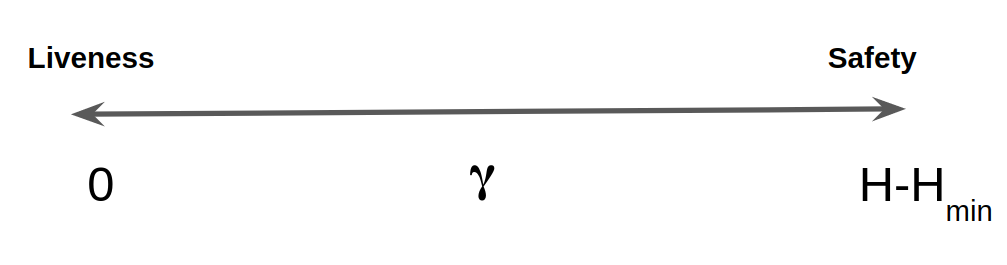
\includegraphics[width=0.6\columnwidth,
	keepaspectratio]{figures/gamma.png}
	\caption{The $\gamma$ parameter versus liveness and safety.}
	\label{fig:gamma_parameter}
\end{figure}

We see from theorem \ref{th:proposed_voting_threshold} that the proposed voting 
threshold is lower bounded by $\frac{H}{2}$. It can be easily proved that it 
could be lower bounded even by $T$, where $T < \frac{H}{2}$. In other words, we 
could have chosen $\tau_V(\gamma) = T + \gamma$ where $0 < \gamma < \mu$ and 
still enjoy the properties of safety and liveness. We have chosen to lower 
bound $\tau_V$ by $\frac{H}{2}$, because we want to honor honest stake 
\emph{majority} and not \emph{minority}. For example, if $T=20\%$ ($H=80\%$) 
and we have 
chosen 
$\tau_V = 25\%$, then even a $30\%$ of honest stake positive votes would be 
enough to approve a result, assuming that the rest $50\%$ of 
the honest stake does not vote, or that their votes are split to $25\%$ reject 
and $25\%$ abstain votes. Since we do not want to allow honest minority to 
control the voting result like this we have decided to lower bound $\tau_V$ by 
$\frac{H}{2}$.

Another important observation is that our analysis is based on the assumption 
that we can have an estimation of the adversary ratio $r$. If it is not 
possible to estimate $r$ with some accuracy, then we could take a worst case 
approach for estimating $r$. From Garay et. al. in \cite{sok}, we know that the 
ratio $r = \frac{T}{T+H} = \frac{T}{100}$ is always upper bounded by the 
theoretical 
adversary tolerance $r_{Th}$ of our consensus protocol, i.e., $r = 
\frac{AdversaryStake}{TotalStake} = \frac{T}{100} < r_{Th}$ (e.g., $r < 1/2 = 
r_{Th}$, or $r < 1/3 = r_{Th}$ etc.).

In table \ref{table:examples}, we provide some examples of the voting threshold 
$\tau_V$ for different values of $\gamma$ and different adversary ratios r.For 
a specific adversary ratio r, as we increase $\gamma$, we require stronger 
honest stake majority, in order to avoid the denial of approval attack. Looking 
at the columns we can see that the voting threshold gradually decreases when r 
increases for a fixed value of $\gamma = 0$. While this is not the case in the 
$\gamma = T$ column, where the threshold increases since it is linearly 
depended on T ($\tau_V = 50 + \frac{T}{2}$). Finally, in the last column, the 
threshold decreases because it is linearly depended on H ($\tau_V = H - 1$) and 
H decreases as r increases.

\begin{table}[h!]
	\centering
	\begin{tabular}{ | c | c | c | c |} 
		\hline
		Adversary ratio r ($r < 1/3 \approx 0.33$) & $\gamma = 0$ & $\gamma = 
		T$ & $\gamma = \frac{H}{2} - 1$ \\ 
		\hline
		$0.1$ & $45\%$ & $55\%$ & $89\%$ \\ 
		$0.2$ & $40\%$ & $60\%$ & $79\%$ \\ 
		$0.3$ & $35\%$ & $65\%$ & $69\%$ \\ 
		\hline
	\end{tabular}
	\caption{Voting threshold values for different $\gamma$ and adversary 
	ratios.}
	\label{table:examples}
\end{table}



\begin{comment}
\begin{theorem}\label{th:proposed_voting_threshold}
	If the voting threshold $\tau_V$ of a voting protocol is defined as:
	\begin{align*}
		&\tau_V(\gamma) = T + \gamma  = 100r + \gamma \\
		&\land\\
		&T < \frac{H}{2} \overset{eq. \ref{eq:H_plus_T}}{\iff} r < \frac{1}{3}\\
		&\land\\
		&0 < \gamma < \mu\\
		&,where\ 0 < \mu \leq \frac{H}{2}\ and\ r = \frac{T}{100}\ is\ the\ 
		adversary\ ratio
	\end{align*}
	then both the safety and liveness properties hold.
	\begin{proof}
		Since 
		\begin{align*}
			&0 < \gamma \iff\\
			&T < T + \gamma \iff\\			
			&T < \tau_V
		\end{align*}
		Also, since
		\begin{align*}
			&\gamma < \mu \iff\\
			&T + \gamma < T + \mu \overset{T < \frac{H}{2}}{\iff}\\
			&T + \gamma < \frac{H}{2} + \mu \iff\\
			&\tau_V < \frac{H}{2} + \mu
		\end{align*}
		Therefore we have proved that $T < \tau_V < \frac{H}{2} + \mu$ and thus 
		based on theorem \ref{th:safety_and_liveness_condition} both safety and 
		liveness properties hold.
	\end{proof}
\end{theorem}

Theorem \ref{th:proposed_voting_threshold} provides a definition of the voting 
threshold that is sufficient for both the safety and liveness properties to 
hold. This holds only when the adversary stake $T < 1/3 \times 100 \approx 
33.33\%$. The $\gamma$ parameter can essentially take values in the range $0 
< \gamma < \frac{H}{2}$ and is always upper bounded by the strength of the 
honest majority result $\mu$. This means that \emph{only} honest majority 
results of strength $\mu > \gamma$ cannot be blocked (i.e., the liveness 
property holds).

For $\gamma$ values close to $0$, we see that $\tau_V$ approaches $T$, where $T 
< \frac{H}{2}$, which means that an honest majority 
result of \emph{any} strength $\mu$ will be approved (i.e., cannot be blocked), 
even if the honest majority is marginal, i.e., just $\frac{H}{2} + 1$. 
Moreover, for such very low values of $\gamma$ even honest minority results 
could be approved in certain cases. For example, assume $T=20\%$ and therefore 
$H = 80\%$. If we choose $\tau_V = 25\%$, then for example, an honest stake 
positive result of $30\%$ could be approved, assuming that the rest $50\%$ of 
the honest stake does not vote, or that their votes are split to $25\%$ reject 
and $25\%$ abstain votes. If we do not want allow such honest stake minority 
results to control the result, we could simply lower bound $\gamma$ by 
$\frac{H}{2}-T$, i.e., $\frac{H}{2}-T \leq	\gamma < \mu$, where $T < 
\frac{H}{2}$. In this case, the voting threshold $\tau_V$ will be lower bounded 
by $\frac{H}{2}$.

On the 
other hand, low values of $\gamma$ that result to low values for the threshold 
$\tau_V$, increase the risk of 
violating the 
safety property, since in the case of a malicious proposal voted in favor by 
the adversary stake T, there are only $\gamma + 1$ positive votes 
missing for the proposal to be approved. So we could say informally that when 
$\gamma$ values are low, liveness is positively impacted, while safety is 
negatively impacted. Inversely, when $\gamma$ is close to $\frac{H}{2}$, then 
$\tau_V$ increases and becomes very difficult to violate safety. However, we 
know that only stake majority results of strength $\mu>\gamma$ cannot be 
blocked and since $\gamma$ is high valued, the set of results that cannot be 
blocked reduces. So we could say informally that when $\gamma$ values are high, 
liveness is negatively impacted, while safety is positively impacted. The 
relation of the $\gamma$ parameter to the safety and liveness properties is 
depicted in figure \ref{fig:gamma_parameter}.

\begin{figure}[h!] %[H]
	\centering
	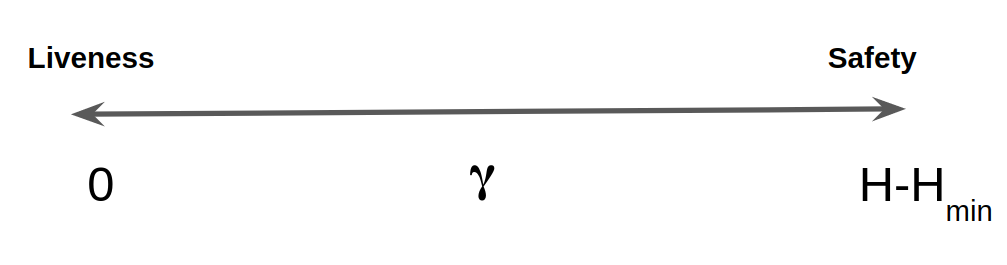
\includegraphics[width=0.6\columnwidth,
	keepaspectratio]{figures/gamma.png}
	\caption{The $\gamma$ parameter versus liveness and safety.}
	\label{fig:gamma_parameter}
\end{figure}

In table \ref{table:examples}, we provide some examples of the voting threshold 
$\tau_V$ for different values of $\gamma$ and different adversary ratios r.For 
a specific adversary ratio r, as we increase $\gamma$, we require stronger 
honest stake majority, in order to avoid the denial of approval attack. Looking 
at the columns we can see that the voting threshold gradually decreases when r 
increases for a fixed value of $\gamma = 0$. While this is not the case in the 
$\gamma = T$ column, where the threshold increases since it is linearly 
depended on T ($\tau_V = 50 + \frac{T}{2}$). Finally, in the last column, the 
threshold decreases because it is linearly depended on H ($\tau_V = H - 1$) and 
H decreases as r increases.

\begin{table}[h!]
	\centering
	\begin{tabular}{ | c | c | c | c |} 
		\hline
		Adversary ratio r ($r < 1/3 \approx 0.33$) & $\gamma = \frac{H}{2}-T$ & 
		$\gamma = 
		T$ & $\gamma = \frac{H}{2} - 1$ \\ 
		\hline
		$0.1$ & $45\%$ & $20\%$ & $54\%$ \\ 
		$0.2$ & $40\%$ & $40\%$ & $59\%$ \\ 
		$0.3$ & $35\%$ & $60\%$ & $64\%$ \\ 
		\hline
	\end{tabular}
	\caption{Voting threshold values for different $\gamma$ and adversary 
	ratios.}
	\label{table:examples}
\end{table}
\end{comment}

\begin{comment}
\subsubsection{On Assumptions and Thresholds}
Lets assume that $H$ is the percent of honest stake and $T$ is the percent of adversarial stake that actively participate in the voting process. From Garay et. al. in \cite{sok}, we know that the ratio $r = \frac{T}{T+H} = \frac{T}{100}$ is upper bounded by the theoretical adversary tolerance $r_{Th}$ of our consensus protocol, i.e., $r = \frac{AdversaryStake}{TotalStake} = \frac{T}{100} < r_{Th}$ (e.g., $r < 1/2 = r_{Th}$, or $r < 1/3 = r_{Th}$ etc.).

Then, the following hold:
\begin{equation} \label{eq1}
T = r \times 100 < 50
\end{equation}
\begin{equation} \label{eq2}
H = (1-r) \times 100 > 50
\end{equation}

Moreover, the stake considered during the tally is the stake that the voters have at that moment. That is, we only consider the stake of the voters at the moment of the tally, without taking into account the stake that the voters had in the moment that the votes were casted. %Therefore, the stake distribution is not known at the moment where the voting takes place, which is a security measure against voters' coercion.\mnote{What do we mean by that? The stake of the voters is known, it is just that we consider the stake distribution at the end of the voting period.}

We know that we have a percent of $H$ honest stake actively voting. Let's assume that we impose a threshold $\tau_V \geq H$. Then, since we need more that $H$ votes for the SU to get approved, then the adversary could block the approval, either by voting 'against', or 'abstain', or by not voting at all. So when the voting threshold exceeds the honest stake percentage participating in the voting process, we risk a denial of approval, even if the honest stake $H$ votes unanimously.


On the opposite side, if we impose a threshold $\tau_V < H$,
, then the adversary could potentially approve a malicious SU, if the honest stake $H$ does not vote a unanimous rejection (i.e., some part of the honest stake votes \say{against}, some other part part votes \say{abstain} and maybe some part (mistakenly) votes positively) and the adversary stake votes positively, so that in total the voting threshold is reached.

Intuitively, when the voting threshold is too low with respect to the honest stake, then we risk the approval of a malicious SU by the adversary stake, while when it is too high, we risk the denial of approval attack. This is a similar (but not identical) situation with the adoption threshold\footnote{The most important difference is that in the case of the adoption threshold, the goal is not just to reach at a decision, we must additionally ensure that a sufficient percent of honest stake has upgraded, in order for the security assumptions of the upgraded ledger to hold.} described in Section \ref{se:informal}.

In general, we assume that the adversary has whatever power is given to him by the threat model of the underlying consensus protocol. Within this scope, we identify two potential attacks.

\paragraph{Malicious Proposal Attack}
The adversary manages with its own stake to approve a malicious proposal.

\paragraph{Denial of Approval Attack}
The adversary manages to block a proposal approved by the honest stake majority.

With respect to the voting threshold $\tau_V$, we have seen that for a software update (either a SIP, or an UP) to get approved the following condition should hold: $stake\ in\ favour > \tau_V$. We provide the following definition:
\begin{definition}
We define as an $\mu$-honest stake majority result (e.g., approval, rejection), a voting result that is voted by more than (or equal) $H/2 + \mu$ percent of votes coming from the honest stake $H$ exclusively, where $0 < \mu \leq H/2$.

If we do not explicitly define $\mu$, then we simply say that we have an honest stake majority result.
\end{definition}
Essentially, an $\mu$-honest stake majority result signifies the strength of a voting result that has been voted by the honest majority. If $\mu = H/2$, then we have a unanimous result from the honest stake $H$. We call $\mu$ the \emph{strength} of an honest stake majority result.

Based on this definition, for our voting mechanism, we set two main security goals:
\begin{itemize}
\item \textbf{Security Goal A (Safety property):} a software update that has 
not achieved an honest stake approval, will never be allowed to pass to the 
next phase in the SU lifecycle, i.e., will not be approved.
\item \textbf{Security Goal B (Liveness property):} a software update that has 
achieved an honest stake majority approval, will be allowed to pass to the next 
phase in the SU lifecycle, i.e., will be approved.
\end{itemize}

Intuitively, failing to achieve the first goal means that we risk the adversary to be able to approve a malicious proposal that is not approved by the honest stake (i.e., some part of the honest stake); and by failing to achieve the second goal, we risk that the adversary might block the approval of a proposal that has been approved by the honest stake majority (i.e., at least half of the honest stake). %We call the latter a \emph{Denial of Approval} attack.

Naturally, in order to avoid the approval of a malicious proposal by the adversary stake $T$, we need a voting threshold $\tau_V > T$. So that the adversary cannot control the result of the voting process with its own stake. Therefore, $\tau_V = T + \delta$, where $\delta > 0$. Without loss of the generality, we choose to express $\delta$ as a fraction of the honest stake $H$. I.e.,
\begin{equation} \label{eq-tau_v}
\tau_V(p) = T + \frac{H}{p},\ p > 1
\end{equation}

We call $p$ the \emph{honest fraction parameter}. If we allowed  $p=1$, then the voting threshold would equal the total stake, but we need  $stake\ in\ favour > \tau_V$ to approve a software update. Therefore, we require that $p>1$. Clearly this condition guards us against the malicious proposal attack, since there will always be a need for some honest stake to vote positively, additionally to the adversary stake, in order to approve a malicious proposal. The smaller the value of the parameter $p$ the more control is handed over to the honest parties. For $1 < p \leq 2$, the control of the decision to approve, or not, a malicious proposal is given to the honest stake majority, since more than half of the honest stake must vote positively. On the contrary, if $p > 2$, then the control of the decision to approve or not a malicious proposal goes to an honest stake minority. Of course, the smaller the percent of honest stake that controls the decision, the more possible is to have a malicious proposal attack.

In Equation \ref{eq-tau_v}, we have expressed the adoption threshold as a function of the honest fraction parameter $p$, which defines the required fraction of the honest stake $H$. In the following theorem we identify what is the necessary and sufficient condition in order for this adoption threshold to satisfy both of the security goals.

\begin{theorem} \label{theorem-adopthresh}
The adoption threshold $\tau_V(p) = T + \frac{H}{p},\ p > 1$ achieves both security goals A and B iff the honest majority strength $\mu$ is $\mu > T + H \times (\frac{1}{p} - \frac{1}{2})$ and the honest fraction parameter $p$ is $1 < p \leq 2$.
\end{theorem}
\begin{proof}
Clearly, for security goal A, in order for the adversary stake not to have the power to vote for a malicious proposal on its own, we need $\tau_V \geq T + \delta$,
where $0 < \delta < H$. In our case, $\delta = \frac{H}{p},\ p > 1$, where $0 < 
\frac{H}{p} < H$. In other words, there will always be the need for a 
fraction of the honest stake $H$ to vote in order to approve a proposal.

For security goal B, we assume that we have an $\mu$-honest stake majority approval for an SU. This means that the specific SU has received a number of $H/2 + \mu$ positive votes from the honest stake, where $0 < \mu \leq H/2$.
The adoption threshold could be lower bounded by $T + H/2$. This results from 
the fact that our threshold should be above $T$, as much as possible, to ensure 
security goal A, but at the same time, we know that we have an honest stake 
majority approval, which by definition means that we have also received more 
that $H/2$ honest positive votes. Therefore,  $\tau_V > T + H/2$. Then, 
equivalently we can wright $\tau_V = T + H/p ,\ 1 < p \leq 2$.

In order for the adversary not to be able to block this approval, of course we need $\tau_V < H/2 + \mu$. But then this also means that $T + H/p < H/2 + \mu$, which means $\mu > T + H \times (\frac{1}{p} - \frac{1}{2})$.
\end{proof}

Intuitively, the closer $p$ gets to $1$ the safer it is with respect to the malicious proposal attack. On the other hand, as $p$ gets smaller, the adoption threshold gets bigger and the more control we give to the adversary stake to block a good proposal. So we need to strike the right balance and choose a value for $p$ (i.e., the right percent of honest stake) that will keep us safe from both attacks. In the lemma that follows we prove that the optimal value of $p$ that achieves both of the above security goals, while requiring the minimum honest majority strength $\mu$, is $2$.

\begin{lemma} \label{lemma-all-in-one}
The optimal voting threshold that achieves both security goals A and B, while requiring the minimum honest majority strength $\mu$, is $\tau_V = T + \frac{H}{2} = 50 \times (r + 1)$ and the necessary and sufficient condition is $T < \mu$.
\end{lemma}
\begin{proof}
From theorem \ref{theorem-adopthresh}, we know that in order for the two security goals to hold we need $\tau_V(p) = T + \frac{H}{p}$ and $\mu > T + H \times (\frac{1}{p} - \frac{1}{2})$ and $1 < p \leq 2$.

For security goal B, since $1 < p \leq 2$, then the component $H \times (\frac{1}{p} - \frac{1}{2}) \geq 0$ and becomes $0$, when $p = 2$ and becomes larger as $p$ gets closer to $1$. This means that the smaller $p$ gets, i.e., for larger fractions of the honest stake, we require a greater strength $\mu$ of an honest stake majority result to avoid the blocking of the adversary. Obviously, the less honest stake is required to avoid the denial of approval attack the better. Therefore, in the range of values $1 < p \leq 2$ the value of $p$ that achieves the minimum strength $\mu$, is the value $p = 2$. In this case, from theorem \ref{theorem-adopthresh} the voting threshold becomes $\tau_V = T + \frac{H}{2}$ and the necessary and sufficient condition for $T$ becomes $T < \mu$.

If $\tau_V = T + \frac{H}{2}$ it is trivial to see that the security goal A is achieved (more that $T$ stake is required for the approval of a proposal).

Finally, for $p=2$, if we substitute $H$ and $T$ from equations \ref{eq1} and \ref{eq2}, we get that $\tau_V = 50 \times (r + 1)$
\end{proof}


%With respect to our two security goals, we provide the following theorems:
%
%\begin{theorem}\label{theorem-v-threshold1}
%if $\tau_V = T + H/p,\ 1 < p \leq 2$, then the security goal A is achieved, i.e., a software update that has not achieved an honest stake majority approval cannot be approved.
%\end{theorem}
%
%\begin{proof}
%Clearly, in order for the adversary stake not to have the power to vote for a malicious proposal on its own, we need $\tau_V \geq T + \delta$, where $0 < \delta \leq H$. According to our security goals, we want to give to the honest stake majority the power to control the result of the voting process. Therefore $\delta$ should be lower bounded by $H/2$, which means that $\tau_V \geq T + H/2$. Then, equivalently we can wright $\tau_V = T + H/p ,\ 1 < p \leq 2$.
%\end{proof}
%
%\begin{theorem}\label{theorem-v-threshold2}
%If $\tau_V = T + H/2,$ and $T < \mu$, then both the security goals A and B are achieved, i.e., a software update that has not achieved an honest stake majority approval cannot be approved and a software update that has achieved an $\mu$-honest stake majority approval cannot be blocked by the adversary stake $T$.
%\end{theorem}
%
%\begin{proof}
%Since $\tau_V = T + H/2,$, therefore $\tau_V = T + H/p, \ p=2$ and we know from theorem \ref{theorem-v-threshold1} that the security goal A holds for this value of $p$.
%Since we have an $\mu$-honest stake majority approval for an SU. This means that the specific SU has received a number of $H/2 + \mu$ positive votes from the honest stake, where $0 < \mu \leq H/2$. In order for the adversary not to be able to block this approval, we need $\tau_V < H/2 + \mu$. But then this also means that $T + H/2 < H/2 + \mu$, which of course means $T < \mu$.
%\end{proof}

%All in all theorem \ref{theorem-v-threshold1} says that the control of a malicious proposal's approval can be under the honest stake majority, if the voting threshold is sufficiently large and in particular it must be $\tau_V \geq T + H/2$. While theorem \ref{theorem-v-threshold2} says that in order for the adversary stake $T$ not to be able to block an $\mu$-honest stake majority result and launch a denial of approval attack, the \emph{strength} of the honest stake majority result $\mu$ must be greater than the adversary stake percent $T$.

All in all, lemma \ref{lemma-all-in-one} says that the control of a malicious proposal's approval can be under the honest stake and at the same time we can avoid the blocking of an $\mu$-honest stake majority approval, with a minimum required strength $\mu$, if $\tau_V = T + \frac{H}{2}$ and $T < \mu$.

\begin{lemma} \label{lemma-unanimous}
If we have a unanimous approval by the honest stake for a software update, then we need also $T < 1/3 \times 100$, in order for this approval not to be able to be blocked by the adversary stake.
\end{lemma}
\begin{proof}
If we have a unanimous approval by the honest stake (i.e., $H$ positive votes from the honest stake), then $\mu = H/2$. In this case, we know from lemma \ref{lemma-all-in-one}, that in order to avoid blocking we need to have $T < \mu$, which means $ T < H/2$ and because of $H = 100 -T$, we get $T < 1/3 \times 100$.
\end{proof}

\begin{lemma}
If $\tau_V = T + H/2 =  50 \times (r + 1)$, then the voting threshold is upper bounded by 75\%, $\tau_V < 75\%$
\end{lemma}
\begin{proof}
Since $\tau_V =  50 \times (r + 1)$ and we know that $r$ is upper bounded by $r_{Th}$. Due to the necessity of the honest majority (according to Garay et al. \cite{sok}), we know that $r_{Th}$ is upper bounded by $0.5$. Then $\tau_V <  50 \times (0.5 + 1) = 75$.
\end{proof}

For example, lets take $\tau_V = T + H/2$. If $T = 30\%$, then $H = 70\%$ and $\tau_V = 65\%$. In this case, only $\mu = 31$-honest stake majority results cannot be blocked (i.e., we need $ \frac{70}{2} + 31 = 66\%$, or more of honest stake positive votes to avoid the denial of approval attack). If we ignored this and just picked a high threshold, like the 95\% used by bitcoin \cite{bitcoin}, then we would enable blocking by the adversary, when we could have a low threshold like 65\% and enjoy safety from blocking by requiring at least 66\% of honest stake positive votes.


In the case where we have an adversary stake percent that is greater, or equal than $1/3 \times 100 \approx 33.33\%$, then even if we have a unanimous honest stake majority approval, according to lemma \ref{lemma-unanimous} the adversary can still launch a denial of approval attack. For example, if $T = 40\%$, then $H = 60\%$ and $\tau_V = 70\%$ and even if all the honest stake votes positively, the adversary can still block the approval.

 To mitigate this risk, as we have already described above, we propose that a denial of approval attack results to a no-majority result, which leads to a revoting process for the specific SU. This revoting can take place a $rv_{no-majority}$ number of times and only after $rv_{no-majority}$ times of a no-majority result the SU will become expired. Therefore, we are limiting the power of the adversary to block a SU, only for a specific voting period and give the chance to the honest stake ($rv_{no-majority}$ number of times) to reconsider its decision and maybe choose to support a candidate SU with a stronger vote.

\end{comment}

\subsection{Delegation} \label{appxdelegation}
Each stakeholder has the right to participate in the software updates protocol of a proof-of-stake blockchain system.
%This participation entails: the submission of update proposals (in the form of SIPs and later as UPs), the approval, or rejection, of SIPs or UPs through a voting process and finally the adoption signaling, when an upgrade has taken place.
In this section, we discuss the delegation of the protocol participation right to some other party. As we will see next, this delegation serves various purposes and copes with several practical challenges.
\subsubsection{Delegation for Technical Expertise}\label{delfortech}
One of the first practical challenges that one faces, when dealing with the decentralized governance of software updates is the requirement of technical expertise, in order to assess a specific software update proposal. Indeed, even at the SIP level, many of the software update proposals are too technical for the majority of stake to understand. Moreover, during the UP approval phase, the approver is called for approving, or rejecting, the submitted source code, which is certainly a task only for experts.

Our proposal for a solution to this problem is to enable delegation for technical expertise. Stakeholders will be able to delegate their right to participate in the update protocol to an \emph{expert pool}. The proposed delegation to an expert pool comprises the following distinct responsibilities:
\begin{itemize}
\item The voting for a specific SIP
\item The voting for a special category of SIPs
\item The voting for any SIP
\item The approval of a specific UP
\item The approval of a special category of UPs
\item The approval of any UP
%\item The adoption signaling for a specific UP
\end{itemize}
As you can see, we distinguish delegation for voting for a SIP document and that for approving an UP. We could have defined delegation for SIP voting to imply also the approval of the corresponding UP. However, since both have a totally different scope, there might be a need to delegate to different expert pools for these two. Indeed, a SIP is an update proposal justification document and the expert who is called to vote for, or against, a specific SIP, must have a good sense of the road-map of the system. On the contrary, the approval of a UP is a very technical task, which deals with the review and testing of a piece of code against some declared requirements (i.e., the corresponding SIP) and has nothing to do with the software road-map.

%We allow voting for a specific SIP/UP, or for \emph{any} SIP/UP. In the former case, the id of the specific SIP/UP must be submitted along with the delegation certificate. In the latter case, if one wants to override the \say{any} delegation and delegate to some other party for a specific SIP/UP, then this is possible via the submission of a new delegation for the specific SIP/UP.
%
%There is also delegation for special categories of SIP/UPs, as well as the delegation for the adoption signaling. These will be the topics that we will describe next.

\subsubsection{Delegation for Specialization} \label{appxdelspecial}
%\nnote{Describe how we use delegation for enabling voting for specialized UPs (e.g., platform specific)}
It is known that there exist special categories of software updates. Let us consider for example, security fixes. It is common sense, that security fixes are software updates that: a) have a high priority and b) require significant technical expertise to be evaluated. Therefore, by having a special expert pool as a \emph{default delegate} for this category of software updates (both SIPs and UPs) enables: a) a faster path to activation and b) sufficient expertise for the evaluation of such SUs. The former is due to the omission of the delegation step in the process and that the evaluation (i.e., voting of SIPs/UPs) will take place generally in shorter times; exactly because this is a specialized and experienced expert pool that deals only with security fixes; we assume that they can do it faster than anybody else.

%There are many different angles (a.k.a. dimensions) by which one can view software updates and distinguish them into different categories. For example, the reason for a SU can be such an angle (i.e., dimension). A SU can be a bug-fix (or security fix), or it can be a change request (or a new feature request). Another dimension is the priority (high/medium/low) of the SU. Furthermore, in blockchain systems, a typical dimension for distinguishing SUs is the impact to the consensus protocol (impact/no-impact). Moreover, for those SUs that impact the consensus protocol, the type of change that they trigger (soft/hard fork) is another dimension. For those SUs that do not impact the consensus protocol another dimension could be, if they are platform specific (e.g., applicable only to Linux, Windows, MacOS etc. versions of the client software).

%All these are valid ways to categorize software updates to certain categories. However, special categories might justify some specialized treatment.
We do not propose any specific set of categories in this paper. However, we do propose that: a) software updates are tagged with a specific category and b) to use delegation for enabling specialized treatment on special categories.

%Let us consider for example security fixes. It is common sense, that security fixes are software updates that: a) have a high priority and b) require significant technical expertise to be evaluated. Therefore, by having a special expert pool as a \emph{default delegate} for this category of software updates (both SIPs and UPs) enables: a) a faster path to activation and b) sufficient expertise for the evaluation of such SUs. The former is due to the omission of the delegation step in the process and that the evaluation (i.e., voting of SIPs/UPs) will take place generally in shorter times; exactly because this is a specialized and experienced expert pool that deals only with security fixes; we assume that they can do it faster than anybody else.
So, for software updates with a special tag, our proposal is, to have \emph{default} specialized expert pools that will participate in the software updates protocol on behalf of the
 %\emph{whole stake}
 delegated stake. Of course, this default delegation based on SU tagging can be overridden. Any stakeholder can submit a different delegation for a specific SIP/UP regardless of its tag.
%Note that the ''any'' delegation described in the previous subsection does not override delegation for specialization.
%What about software updates without a special tag? These will be the topic of discussion of the next subsection.

\subsubsection{Default Delegation for Availability}\label{defaultdel}
Blockchain protocols based on the Proof-of-Stake (PoS) paradigm are by nature dependent on the active participation of the digital assets' owners --i.e., stakeholders-- (Karakostas et. al. \cite{stakepools}). Practically, we cannot expect stakeholders to continuously participate actively in the software updates protocol. Some users might lack the expertise to do so, or might not have enough stake (or technical expertise) to keep their node up-and-running and connected to the network forever.

One option to overcome this problem, which is typical in PoS protocols, is to enable stake representation, thus allowing users to delegate their participation rights to other participants and, in the process, to form
\say{stake pools}(\cite{stakepools}). The core idea is that stake pool operators are always online and perform
the required actions on behalf of regular users, while the users retain the ownership of their
assets (\cite{stakepools}).

In this paper, we propose to utilize the stake pools mechanism for our software updates protocol in tandem with the consensus protocol. In particular, we propose to allow each stakeholder to define a default delegate for participating in the software updates protocol from the list of available stake pools that participate in the core consensus protocol. This will be a \say{baseline} representative of each stakeholder to the software updates protocol, just for the sake of maintaining the participation to the protocol at a sufficient level and minimizing the risks of non-participation. This delegate will coincide with the delegate for the participation in the consensus protocol. A stakeholder will be able at any time to override this default delegation. A delegation to an expert pool for a specific software update, or a specific category of software updates, due to specialization, described in the previous section, will override the default delegation to a stake pool.
%Moreover, adoption signaling simply follows the delegation of the proof-of-stake consensus protocol and ignores delegation to expert pools. This is because blocks are generated in practice by the stake pools, then these should be also responsible for the adoption signaling as well.

%Therefore,  all software updates without a special category tag that have not been included into an explicit delegation certificate, will be managed (by default delegation) by the same stake pool that the stakeholder has delegated to run the  proof-of-stake consensus protocol. This will allow the stakeholder to be able to abstain from the software updates protocol, for periods of time, without causing a problem. This delegation to stake pools has also another advantage that we discuss next.

%We have seen that one of the responsibilities of a stakeholder that participates in the software updates protocol, at the activation phase, is to signal the adoption of a UP. This signal is placed within each generated block after the node upgrades.
%In addition, we know that in a proof-of-stake consensus protocol blocks are generated by the stakeholders (with possibility proportional to their stake) and in a more realistic setting by the stake pools, which have been delegated to do so. So in practice, the stake pools are called for signaling the adoption event, merely because they are the block issuers. Therefore, the choice of stake pools as the default delegates for the software updates protocol, fits nicely with the fact that stake pools will be responsible for signaling adoption anyway. %If a stakeholder has not delegated his participation to the proof-of-stake consensus protocol and is chosen to generate a block, then he/she will also be responsible for signaling the adoption of a specific UP.
%In other words, adoption signaling simply follows the delegation of the proof-of-stake consensus protocol and ignores delegation to expert pools.

\subsubsection{Delegation Mechanics}
For the realization of the stake pool delegation mechanism that we described above, we closely follow the work of Karakostas et al. \cite{stakepools}, so we refer the interested reader to this work for all the relevant details.
In this subsection, we would like to focus
on the most basic mechanics (i.e., technical details) that will enable such a delegation mechanism to work. Please note that many of our ideas are based on the design of the delegation mechanism for the Cardano blockchain system \cite{deldesign}. %Due to space limitations, we have moved the delegation mechanics to the appendix.
\paragraph{Staking keys.}
Following the Karakostas et. al. \cite{stakepools} approach, we separate for each address the control over the movement of funds (i.e., executing common transactions, such as payments) and that over the right for participation in the proof-of-stake protocol and consequently, in the software updates protocol, due to the ownership of stake. Intuitively, this separation of control is necessary, since we only want to delegate the management of stake to some other party, by means of participation in the software updates protocol and not the management of the funds owned by this stake. This is achieved in practice by assuming that each address consists of two pair of keys: a) a \emph{payment key pair} $K^p = (skp,vkp)$ and b) a \emph{staking key pair} $K^s = (sks, vks)$. With the former a stakeholder can receive and send payments, while with the latter a stakeholder can participate in the proof-of-stake consensus protocol and in the software updates protocol. $skp$ and $sks$ are the secret keys for signing, while $vkp$ and $vks$ are the public keys used to verify signatures.

\subsubsection*{Stake Delegation}
In its simplest form, delegation of stake from some party A to another party B (typically a stake pool) for participation in the proof-of-stake consensus protocol, also delegates the right for participation in the software updates protocol as well. The rationale of this has been described in Subsection \ref{defaultdel} and it holds only on the assumption that there is no explicit delegation to some expert pool. So in the rest of this text, when we refer to stake delegation, we mean for the participation in both the proof-of-stake consensus protocol and the software updates protocol, unless an explicit statement is made for delegation to an experts pool.

At its core, the delegation of stake to some other party, essentially requires two things: a) stake registration and b) issuance of a delegation certificate:

\paragraph{Stake key registration.}
This step is a public declaration of a party that it wishes to exercise its right for participation in the proof-of-stake protocol, due to its ownership of stake. In order for a stakeholder to exercise these rights, he/she must first issue a stake key registration certificate. This is a signed message stored in the metadata (i.e., Payload) of a transaction (see Appendix~\ref{se:bcabstraction}) and thus it is published to the blockchain. The key registration certificate must contain the public staking key $vks$, and the signature of the text of the transaction $m$ by the staking private key $sks$, which is the rightful owner of the stake. In other words, the key registration certificate $r$ is the pair: $r = (vks, \sigma_{sks}(m))$. The signature $\sigma$ of the certificate, authorizes the registration and  plays the role of a witness.
%Interestingly, it also prevents against a certificate replay attack. In particular, since the certificate includes a signature on a specific transaction text, then this certificate is bound forever with the specific transaction, and just like in UTxO accounting blockchains, a transaction cannot be replayed (a UTxO can be only spent once), similarly a certificate cannot be replayed either. For account based blockchains there are other approaches that one can follow, in order to prevent a replay attack, such as the \emph{address whitelist} proposed in Karakostas et. al. \cite{stakepools}.
Symmetrically, there is also a de-registration certificate for a stake key, which is a declaration that a party no longer wishes to participate in the proof-of-stake protocol.

\paragraph{Delegation registration.}
In order to register the delegation of stake from one party (source) to another (target), a delegation certificate must be issued and posted to the blockchain by the source party. This certificate publicly announces to the network that the source party wishes to delegate its stake right (for participation in the proof-of-stake protocol) to the target party and this is recorded forever in the immutable history of the blockchain.
At a minimum, a delegation certificate consists of the following information:
$$
(H(vks_{source}), H(vks_{target}), \sigma_{sks_{source}}(m))
$$
Where, $H(vks_{source})$ is the hash of the source party's public staking key, $H(vks_{target})$ is the hash of the target party's public staking key and $\sigma_{sks_{source}}(m)$ is the signature of the text $m$ of the transaction (within which the delegation certificate is embedded) by the source party's private staking key $sks_{source}$, which authorizes the certificate and plays the role of a witness (see Appendix~\ref{se:bcabstraction} for a formal definition of the signature scheme).

If at some point, the source party wishes to re-delegate to some other party, or even to participate in the protocol on its own, then it must simply issue a new delegation certificate. For self-participation in the protocol, a party must issue a delegation certificate to its own \emph{private stake pool}\footnote{A \emph{private stake pool} is a trivial case of a stake pool. By treating self-staking as a special case of stake pool delegation is a design decision for the sake of simplicity \cite{deldesign}.}. If the source staking key is de-registered, then the delegation certificate is revoked.

\subsubsection*{Delegation to an Expert Pool}
We have seen that by default, the participation right in the software updates protocol is delegated to the stake pool that the delegation for participation in the proof-of-stake consensus protocol has taken place. So by default, some stake pool will participate in the software updates protocol. Next, we will discuss the case where a stakeholder wants to override the default behavior and explicitly delegate to an expert pool.

An expert pool is an entity consisting of one or more experts, who are willing to participate in the software updates protocol as delegates of other stakeholders. Their main task is to vote for (or against) SIPs and to approve (or reject) UPs. We call them \say{experts}, because they need to have sufficient technical expertise, in order to evaluate a software update.

In order to enable delegation to an expert pool, we extend the delegation certificate presented above, with additional information. In particular, a delegation certificate to an expert pool is defined as the following tuple:
\begin{align*}
(H(vks_{source}), \\
 H(vks_{target}), \\
 \sigma_{sks_{source}}(m), \\
 SU_{Flag}, \\
 H(<SIP/UP>), \\
 <category>)
\end{align*}

In this case, the $H(vks_{target})$ is the hash of the public staking key of the expert pool. We have extended the delegation certificate to include a boolean flag $SU_{Flag}$, which denotes, if the delegation pertains to a SIP, or an UP. We have explained previously (see subsection \ref{delfortech}), the rationale for distinguishing the delegation for these two. Finally, the hash $H(<SIP/UP>)$ is the hash of the content of the SIP, or UP, in question and plays the role of the unique id for this SIP, or UP respectively. Note that if instead of a specific SIP/UP id, a special value is provided for this field (e.g., '*'), then this corresponds to a delegation for \emph{any} SU of this type (SIP or UP). Finally, if the SU id field is empty (or $NULL$, it depends on the implementation), then we take into account the last field, which specifies the \emph{category} of the SU (e.g., \say{security-fix}, \say{linux-update}, etc.) that, we wish to delegate for. This will be a simple string value chosen from a fixed set of values (a list of acknowledged SU categories).

In summary, with this certificate, a party can delegate its participation right in the software updates protocol to an expert pool: a) for a specific software update (SIP or UP), b) for a specific category of software updates, or c) for any software update. Of course, in order for this delegation registration to be valid, the target expert pool must have been appropriately registered first in the blockchain. This is the topic to be discussed next.

\subsubsection*{Expert Pool Registration}
In order for someone to publicly announce his/her intention to play the role of an expert, or equivalently, to run an expert pool, two things are required: a)to issue an expert pool registration certificate and b)to provide appropriate \emph{metadata} describing the expert pool.

\paragraph{Expert pool registration certificate.}
The certificate contains all the information that is relevant for the execution of the protocol. At its most basic form this certificate comprises the following:
\begin{itemize}
\item $vks_{expool}$: This is the public staking key of the expert pool. This must be used as the target public key in the delegation certificate, as discussed in the previous subsection.

%\item $[H(vks_{sup_1}), H(vks_{sup_2}), ...,H(vks_{sup_p})] $: A list of $p$ public staking key hashes that aggregate to $P$ total stake. This is called the \emph{pledged stake} of the expert pool and is provided by some stakeholders that we call the \emph{expert pool supporters}. An expert pool registration must be backed up by some (pledged) stake $P$. This is simply a promise made by the expert pool that the pool will receive at least this minimum support by the stake of the supporters. For an expert pool to participate in the software updates (SU) protocol and get rewarded for this, it must be delegated at least $P$ stake from these $p$ stakeholders. If this threshold $P$ is not met (i.e., the pool is delegated less stake than $P$ from the list of $p$ stakeholders mentioned in the certificate), then no participation in the software updates protocol is allowed and thus, no rewards will be payed to the Expert pool. Note that this list in this certificate is not a delegation. The pledged stake must explicitly declare the delegation via issuing distinct delegation certificates, as described above.

\item $(<URL>, H(<metadata>))$: A URL pointing to the metadata describing the expert pool and a content hash of these metadata. The URL points to some storage server and the hash of the content retrieved must match the one stored in the certificate for the pool registration to be considered as valid.

%\item $[\sigma_{sks_{expool}}(m),\sigma_{sks_{sup_1}}(m),...,\sigma_{sks_{sup_p}}(m)]$: The certificate must be authorized by the signature $\sigma$ of the expert pool $sks_{expool}$ and by all the $p$ supporter stakeholders $sks_{sup_i}, i \in [1,p]$, on the text $m$ of the transaction that includes the certificate.

\item $\sigma_{sks_{expool}}(m)$: The certificate must be authorized by the signature $\sigma$ of the expert pool $sks_{expool}$ on the text $m$ of the transaction that includes the certificate.

\end{itemize}

Symmetrically, there should be also an \emph{expert pool retirement certificate} for allowing an expert pool to cease to operate. This should include the public staking key of the expert pool, as well as a time indication (e.g., expressed in block number, or an epoch number etc.) of when the pool will cease to operate.

\paragraph{Expert pool metadata.}
The expert pool metadata are necessary information that describe sufficiently an expert pool, so as the stakeholders community can decide, which expert pool to choose for their delegations. Typically, this information will be displayed by the wallet application, in order to assist the users to select the expert pool of their choice. Examples of useful information to be included in the expert pool metadata are the name of the pool, a short description, the area of expertise, the years of expertise, preferences to specific SU categories, URLs to sites that exhibit the claimed experience and in general any information that can help the stakeholders to choose the appropriate delegate for the right software update.

%\paragraph{Pledged stake rationale.}
%In a centralized setting, a new expert pool, in order to establish a certain level of trust on its credentials from the community of stakeholders, would typically provide some reference/certification from a trusted third party authority. In the decentralized approach, the role of this trusted party that certifies for a new expert pool is assumed by the \emph{supporters stake}. In other words, the \emph{pledged stake} is the stake that supports a new expert pool on registration. This stake is beyond the stake that might (or might not) be owned by the expert pool staking key. It is a way for some of the stake to say that we trust this new expert pool and we are willing to support it by delegating our stake to it. It is therefore, a promise for a minimum of stake delegation to be received from the beginning of operation of the expert pool. It is also a hard prerequisite for allowing the participation of the expert pool in the software updates protocol. Conveniently, it also prevents from a specific type of attack, namely a sybil attack, as we will discuss briefly.

\subsection*{Miscellaneous Considerations on Delegation}

\paragraph{Chain delegation.}
%\nnote{Do we allow chain delegation? Can a stake pool delegate further to some other party?}
Chain delegation is the notion of having multiple certificates chained together, so that the source
key of one certificate is the delegate key of the previous one. In principle there is no reason to prevent the formation of delegation chains. However, an implementation of this proposal must take into account the possibility to form (deliberately or by accident) delegation cycles. This means that a target delegate ends up to be one of the sources. In this case, the delegation is essentially canceled and the system should detect it and prevent it pro-actively.
%In principle, we could allow chain delegation with the following restrictions:
%\begin{itemize}
%\item no cycles allowed
%\item ''Any'' delegation is not allowed by expert pools. (is similar in concept with subcontracting in a project. A subcontractor cannot assume the whole project, only a part of it, otherwise there is no role for the prime contractor).
%\end{itemize}

%\subsubsection*{Security Considerations}

\paragraph{Certificate replay attacks.}
For all our certificates, namely: stake key registration, delegation registration and expert pool registration, we have provided signatures of the text of the encompassing transaction (the certificates are included as transaction metadata), signed by the party(ies) authorized to issue the certificate. This is a design choice made in \cite{deldesign} that prevents against a certificate replay attack. In this attack, an attacker re-publishes an old certificate, in order for example to change a delegation to a new expert pool. In particular, since the certificate includes a signature on a specific transaction text, then this certificate is bound forever with the specific transaction, and just like in blockchains with a UTxO accounting model, a transaction cannot be replayed (a UTxO can be only spent once), similarly the specific certificate cannot be replayed either. For account based blockchains there are other approaches that one can follow, in order to prevent a replay attack, such as the \emph{address whitelist} proposed in Karakostas et. al. \cite{stakepools}, where the transaction that includes the certificate must be issued from a specific whitelisted address. Of course there are other common solutions like the counter-based mechanism (known as the \emph{nonce}) used in Ethereum \cite{ethereum}.

%\paragraph{Sybil attacks.}
%The attack in this case has to do with an adversary who tries to register too many expert pools, in order to gain control of the stake via delegations. The pledged stake described above provides an incentive-based protection mechanism against this type of attack, which has been proposed in Bruenjes et. al. \cite{incentives} and also is described in Kant et. al. \citep{deldesign}. In particular, the commitment of specific stake from the expert pool supporters, in the form of the pledged stake, which is published and stored forever in the blockchain, prevents (indirectly) an adversary to register too many expert pools. Moreover, the fact that the reward of the expert pool could be proportional to the pledged stake, de-incentivizes adversaries to try to register many expert pools with a very small pledged stake.

\paragraph{Identity theft.}
Significant expertise on difficult technical issues is not a skill that is easy to acquire. Moreover, experience comes after a long period (probably many years) of struggle with technical issues. Therefore, real specialists on a technical domain are hard to find and for this reason they are invaluable. Typically, these experts are well-known and well-respected figures in the community. Therefore, such a well-known expert is expected to receive a significant amount of delegations, if he/she chooses to register an expert pool. This fact makes expert pool registration susceptible to identity theft. This is the case where an expert pool falsely claims to be the famous \say{expert A}, just for the sake of receiving the delegations drawn from the fame of the expert. This identity assurance problem is external to the software updates protocol and also to the underlying consensus protocol and thus some out-of-band solution could be adopted. For example, a famous expert, could post his/her public key (or its fingerprint) to social media, so that the people who follow him/her, will know, which is the genuine key that they can delegate to. Of course, other similar in concept, solutions can be exploited as well. However at the end of the day, in a decentralized setting, it is the stake via delegation that will be the ultimate judge of an expert pool.

%\subsection{Fees and rewards}
%\subsubsection{Fees}
%\begin{itemize}
%\item Describe the events of the protocol that are implemented as transactions.
%\item Who are these transactions paying? The treasury system?
%\item Fees prevent DoS attacks
%\end{itemize}

%\subsubsection{Rewards}
%The ideation phase (treasury system) elects some project to fund. In the budget of this project there a portion for the reward of voters and approvers (who might be stake pools or expert pools)
%The reward schemes must be based on \cite{incentives} to guarantee that we will end up with k pools, instead of only one big one.
%Rewards $r(s,p)$ for expert pools will be dependent on the total stake $s$ controlled by the pool and on the pledged stake $p$.
